\documentclass[]{article}



\usepackage{graphicx,forloop,caption,subcaption,float,hyperref,arrayjob,listings,color,booktabs,mathtools}
\usepackage{pdfpages}
\usepackage[margin=1.2in]{geometry}
\usepackage{amsmath}
\usepackage{multirow}
%vhdl code
\definecolor{dkgreen}{rgb}{0,0.6,0}
\definecolor{gray}{rgb}{0.5,0.5,0.5}
\definecolor{mauve}{rgb}{0.58,0,0.82}

\DeclareMathOperator*{\argmin}{\arg\!\min}
\newcommand{\rom}[1]{\uppercase\expandafter{\romannumeral#1}}

\lstset{frame=tb,
  language=VHDL,
  aboveskip=3mm,
  belowskip=3mm,
  showstringspaces=false,
  columns=flexible,
  basicstyle={\small\ttfamily},
  numbers=none,
  numberstyle=\tiny\color{gray},
  keywordstyle=\color{blue},
  commentstyle=\color{dkgreen},
  stringstyle=\color{mauve},
  breaklines=true,
  breakatwhitespace=true
  tabsize=3
}

%matlab code
\lstset{frame=tb,
  language=Matlab,
  aboveskip=3mm,
  belowskip=3mm,
  showstringspaces=false,
  columns=flexible,
  basicstyle={\small\ttfamily},
  numbers=none,
  numberstyle=\tiny\color{gray},
  keywordstyle=\color{blue},
  commentstyle=\color{dkgreen},
  stringstyle=\color{mauve},
  breaklines=true,
  breakatwhitespace=true
  tabsize=3
}


% Title Page
\title{UCLA\\EE230B\\Digital Communication Design Project\\Step 4 Report}
\author{Alican Salor 404271991 \\  \href{mailto:alicansalor@ucla.edu}{alicansalor@ucla.edu} \\ \\
Darren Reis 804359840 \\
\href{mailto:darrer.r.reis@gmail.com}{darren.r.reis@gmail.com} }


\begin{document}
\maketitle

\newpage
\tableofcontents

\newpage
\section{Background}
\label{sec:background}
This step of the project introduces complications from using computers and digital methods to analyze analog signals.  Data conversion, the process of taking a continuous signal and descretizing it, can lead to additional and sometimes catastrophic errors.\\

Recall, digital signals are quantized into samples, discrete points in time.  Conversely, an analog signal has a continuous value.  Going from one to the other requires a converter.  To take an analog signal and digitize it, an Analog-to-Digial Converter (A/D) is used.  Both types of signals are shown in Figure~\ref{fig:digitization}.  There is a wrinkle: the rate of conversion is critical to preserving the information.  By the Nyquist-Shannon Sampling Theorem (\ref{eq:nyquist}), the sampling frequency must be at least twice the highest frequency in the signal.  Without reaching this frequency, the samples can wrongfully convey a lower frequency signal, alias, of the true signal.  This is shown in Figure~\ref{fig:alias}.  

\begin{align}
\label{eq:nyquist}
f_s \geq 2 f_{max}
\end{align}


\begin{figure}[h]
        \centering
        \begin{subfigure}[b]{0.4\textwidth}
                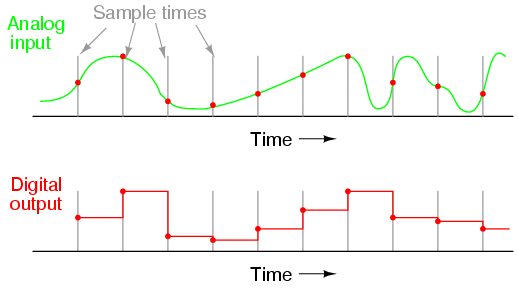
\includegraphics[width=\textwidth]{digitization.png}
                \caption{Analog and Digital signals}
                \label{fig:digitization}
        \end{subfigure}%
        \qquad \quad %add desired spacing between images, e. g. ~, \quad, \qquad etc.
          %(or a blank line to force the subfigure onto a new line)
        \begin{subfigure}[b]{0.5\textwidth}
                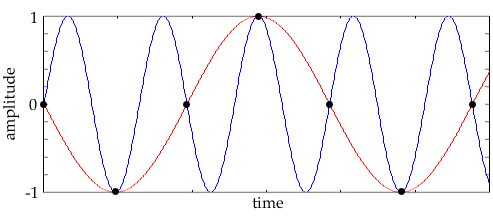
\includegraphics[width=\textwidth]{aliasing.jpg}
                \caption{Aliasing \label{fig:alias} \cite{aliasing}}
                \label{fig:alias}
        \end{subfigure}
        \caption{Digital Conversion \label{fig:digitize}}
\end{figure}

\section{System}
\label{sec:system}
The system simulation model is shown in Figure~\ref{fig:step4}.  As from Step 1, randomly generated bits [Appendix~\ref{app:random_bit_generator}] are converted into symbols [\ref{app:bittosym}] and then upsampled by adding in zeros [\ref{app:impulse_train}].  The result is then is run through a Square Root Raised Cosine (SRRC) pulse shape filter [\ref{app:sqrt_raised_cosine}].  This shaping improves the resistance of the sequence to intersymbol interference (ISI).  The output of this filter is fed into a Digital-to-Analog Converter (DAC).  A DAC takes the digital samples and zero-order holds them at a constant voltage, creating an analog signal [Appendix~\ref{app:da},~\ref{app:zero}].  \\

After the digitizer, a reconstruction filter (also sometimes called an anti-imaging filter) bandlimits the analog waveform output from the DAC.  The high frequency content contained in the stair-case digital signal is undesirable since it can create aliasing of wrongfully high frequency waves.  To avoid this, the Low Pass Filter is used for the reconstruction.  Ours is modeled as a Butterworth filter, or a maximally flat magnitude filter \cite{butter}.  The aim of the filter is to have uniformly flat passband frequency response and roll to zero in the stopband.  As with all filters, the cutoff frequency parameter sets the bands and the order of the filter determines the roll-off of the frequency response in the stopband.  We used a fourth order Butterworth so that the roll-off was $80 \mathtt{\frac{dB}{dec}}$.  We set the cutoff frequency to BLAH BLAH $\mathtt{Hz}$. The interior workings of the filter are not pertinent to this project, so the code in Appendix~\ref{app:butterworth} uses built-in MATLAB functions.  \\

After passing through the reconstruction filter, the analog signal is  sent through a real world channel, modeled by gain and additive white Gaussian noise [Appendix~\ref{app:awgn_channel}].\\

\begin{figure}[H]
\centering
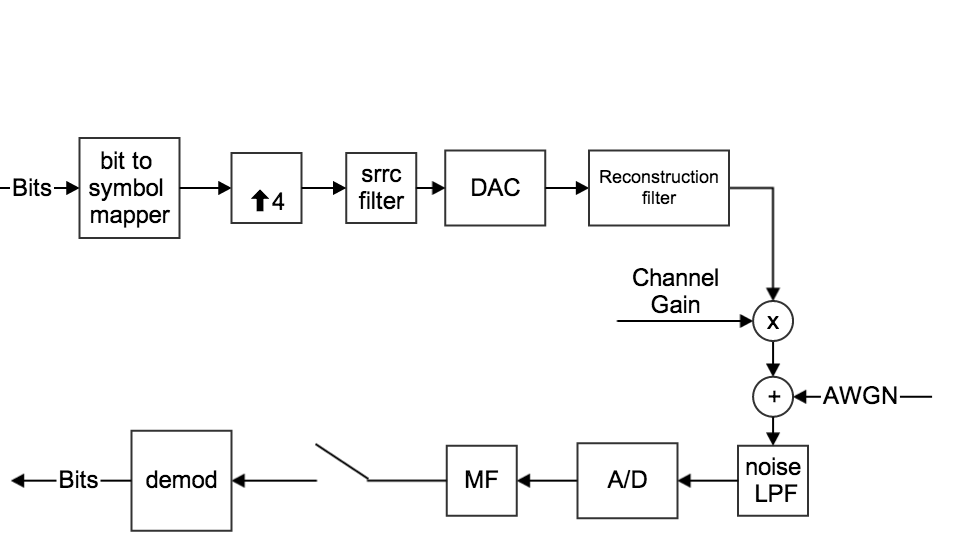
\includegraphics[width=\textwidth]{step4.png}
\caption{Block Diagram of Step 4 system setup\label{fig:step4}}
\end{figure}

To bring the analog back to the digital world, an Analog-to-Digital converter (A/D) is used [Appendix~\ref{app:ad}].  However, just like before, the conversion is improved by the use of a filter.  An anti-aliasing low-pass filter constrains, or band limits, the channel noise before entering the A/D.  In this setting, the LPF protects against aliasing of high frequency content being recorded at the lower frequency.  We use the same Butterworth filter to accomplish this function.\\

The end of the simulation model is identical to the process in Step 1: a matched filter to the SRRC picks out the symbols from the noisy received signal.  Afterwards, a sampler recovers [Appendix~\ref{app:sampler}] the symbols before a demodulator converts the symbols back into bits [\ref{app:dblocks}].  

\section{Experiments}
\label{sec:experiments}


\section{Step 4 Results}
\label{sec:results}
In the following sections the results of the simulations of a system using QPSK modulation and Costas Loop or Decision Directed Recovery Loop for phase/frequency offset recovery. The results are interpreted afterwards in the conclusion section.

%\subsection{QPSK with Decision Directed Recovery}
%\subsubsection{Transience of Phase Recovery}
%\begin{figure}[H]
%\centering
%\hspace*{-2cm}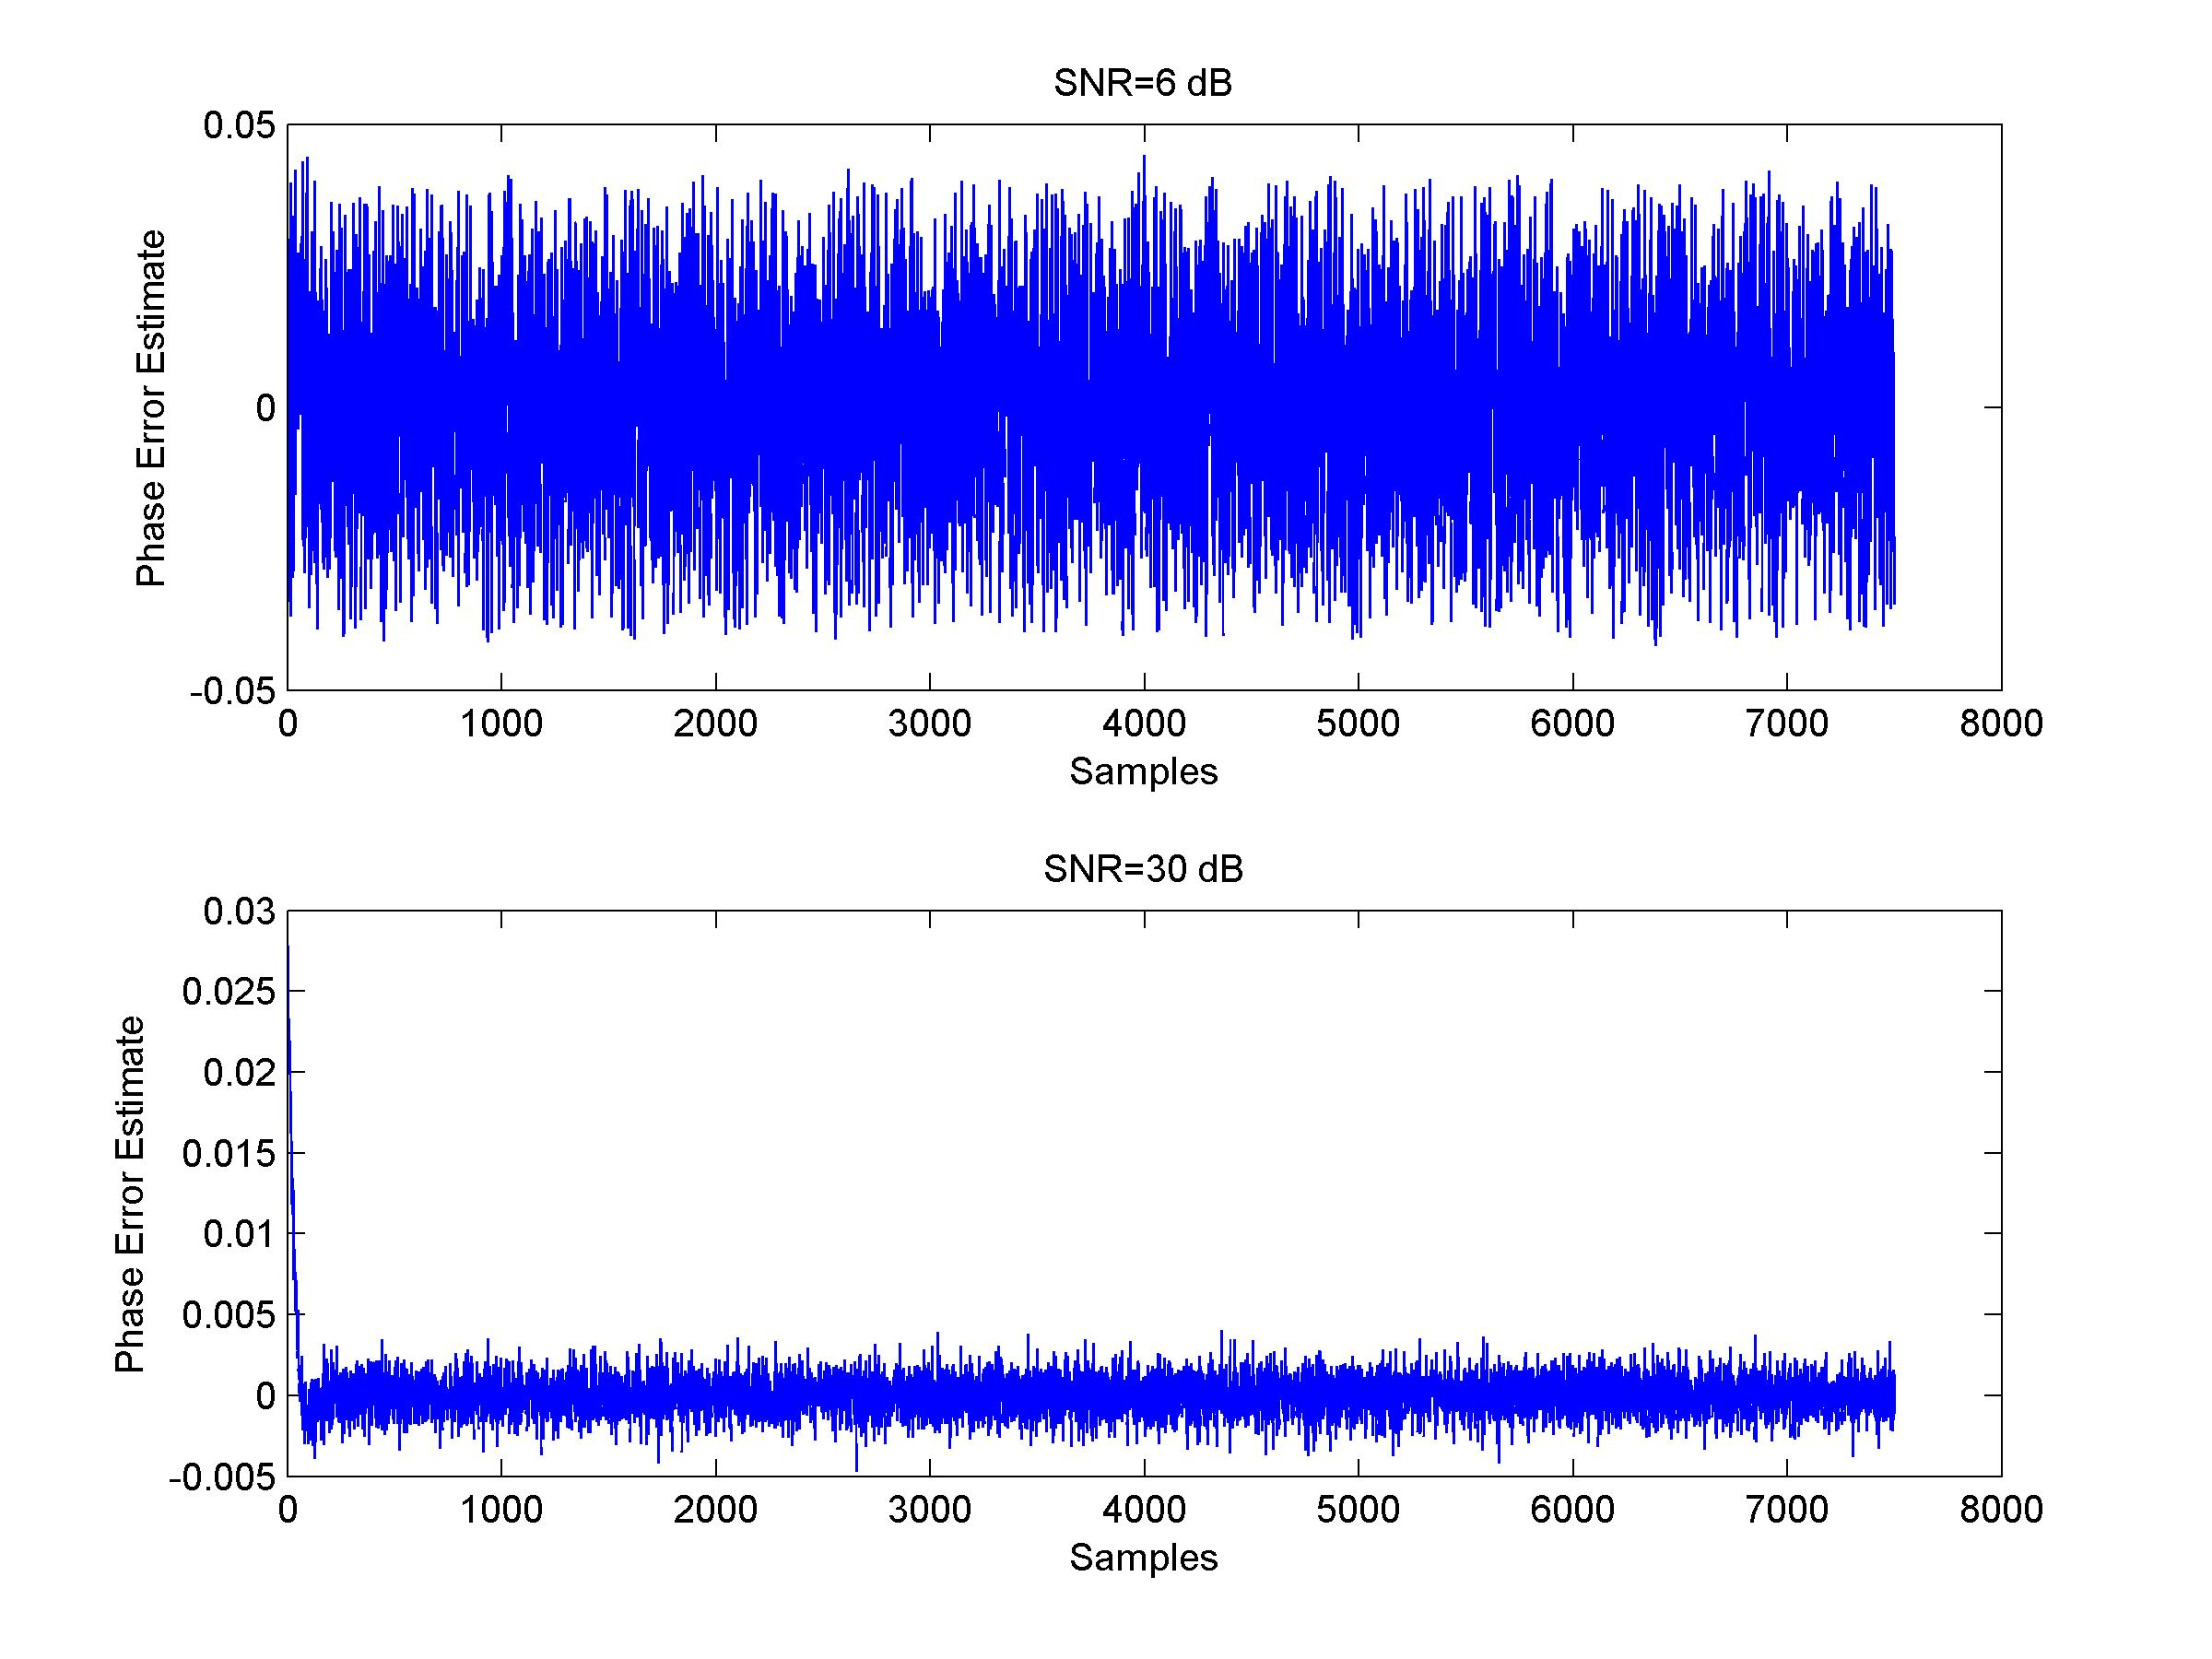
\includegraphics[width=0.7\textwidth]{qpLoopFilterpo_ddr1.jpg}
%\caption{The loop filter output of the Decision Directed Recovery Loop for an input signal with 30 degrees phase offset \label{fig:ddrTransphase}}
%\end{figure}
%
%
%\subsubsection{Constellation Plots  for Phase Recovery}
%\begin{figure}[H]
%\centering
%\hspace*{-2cm}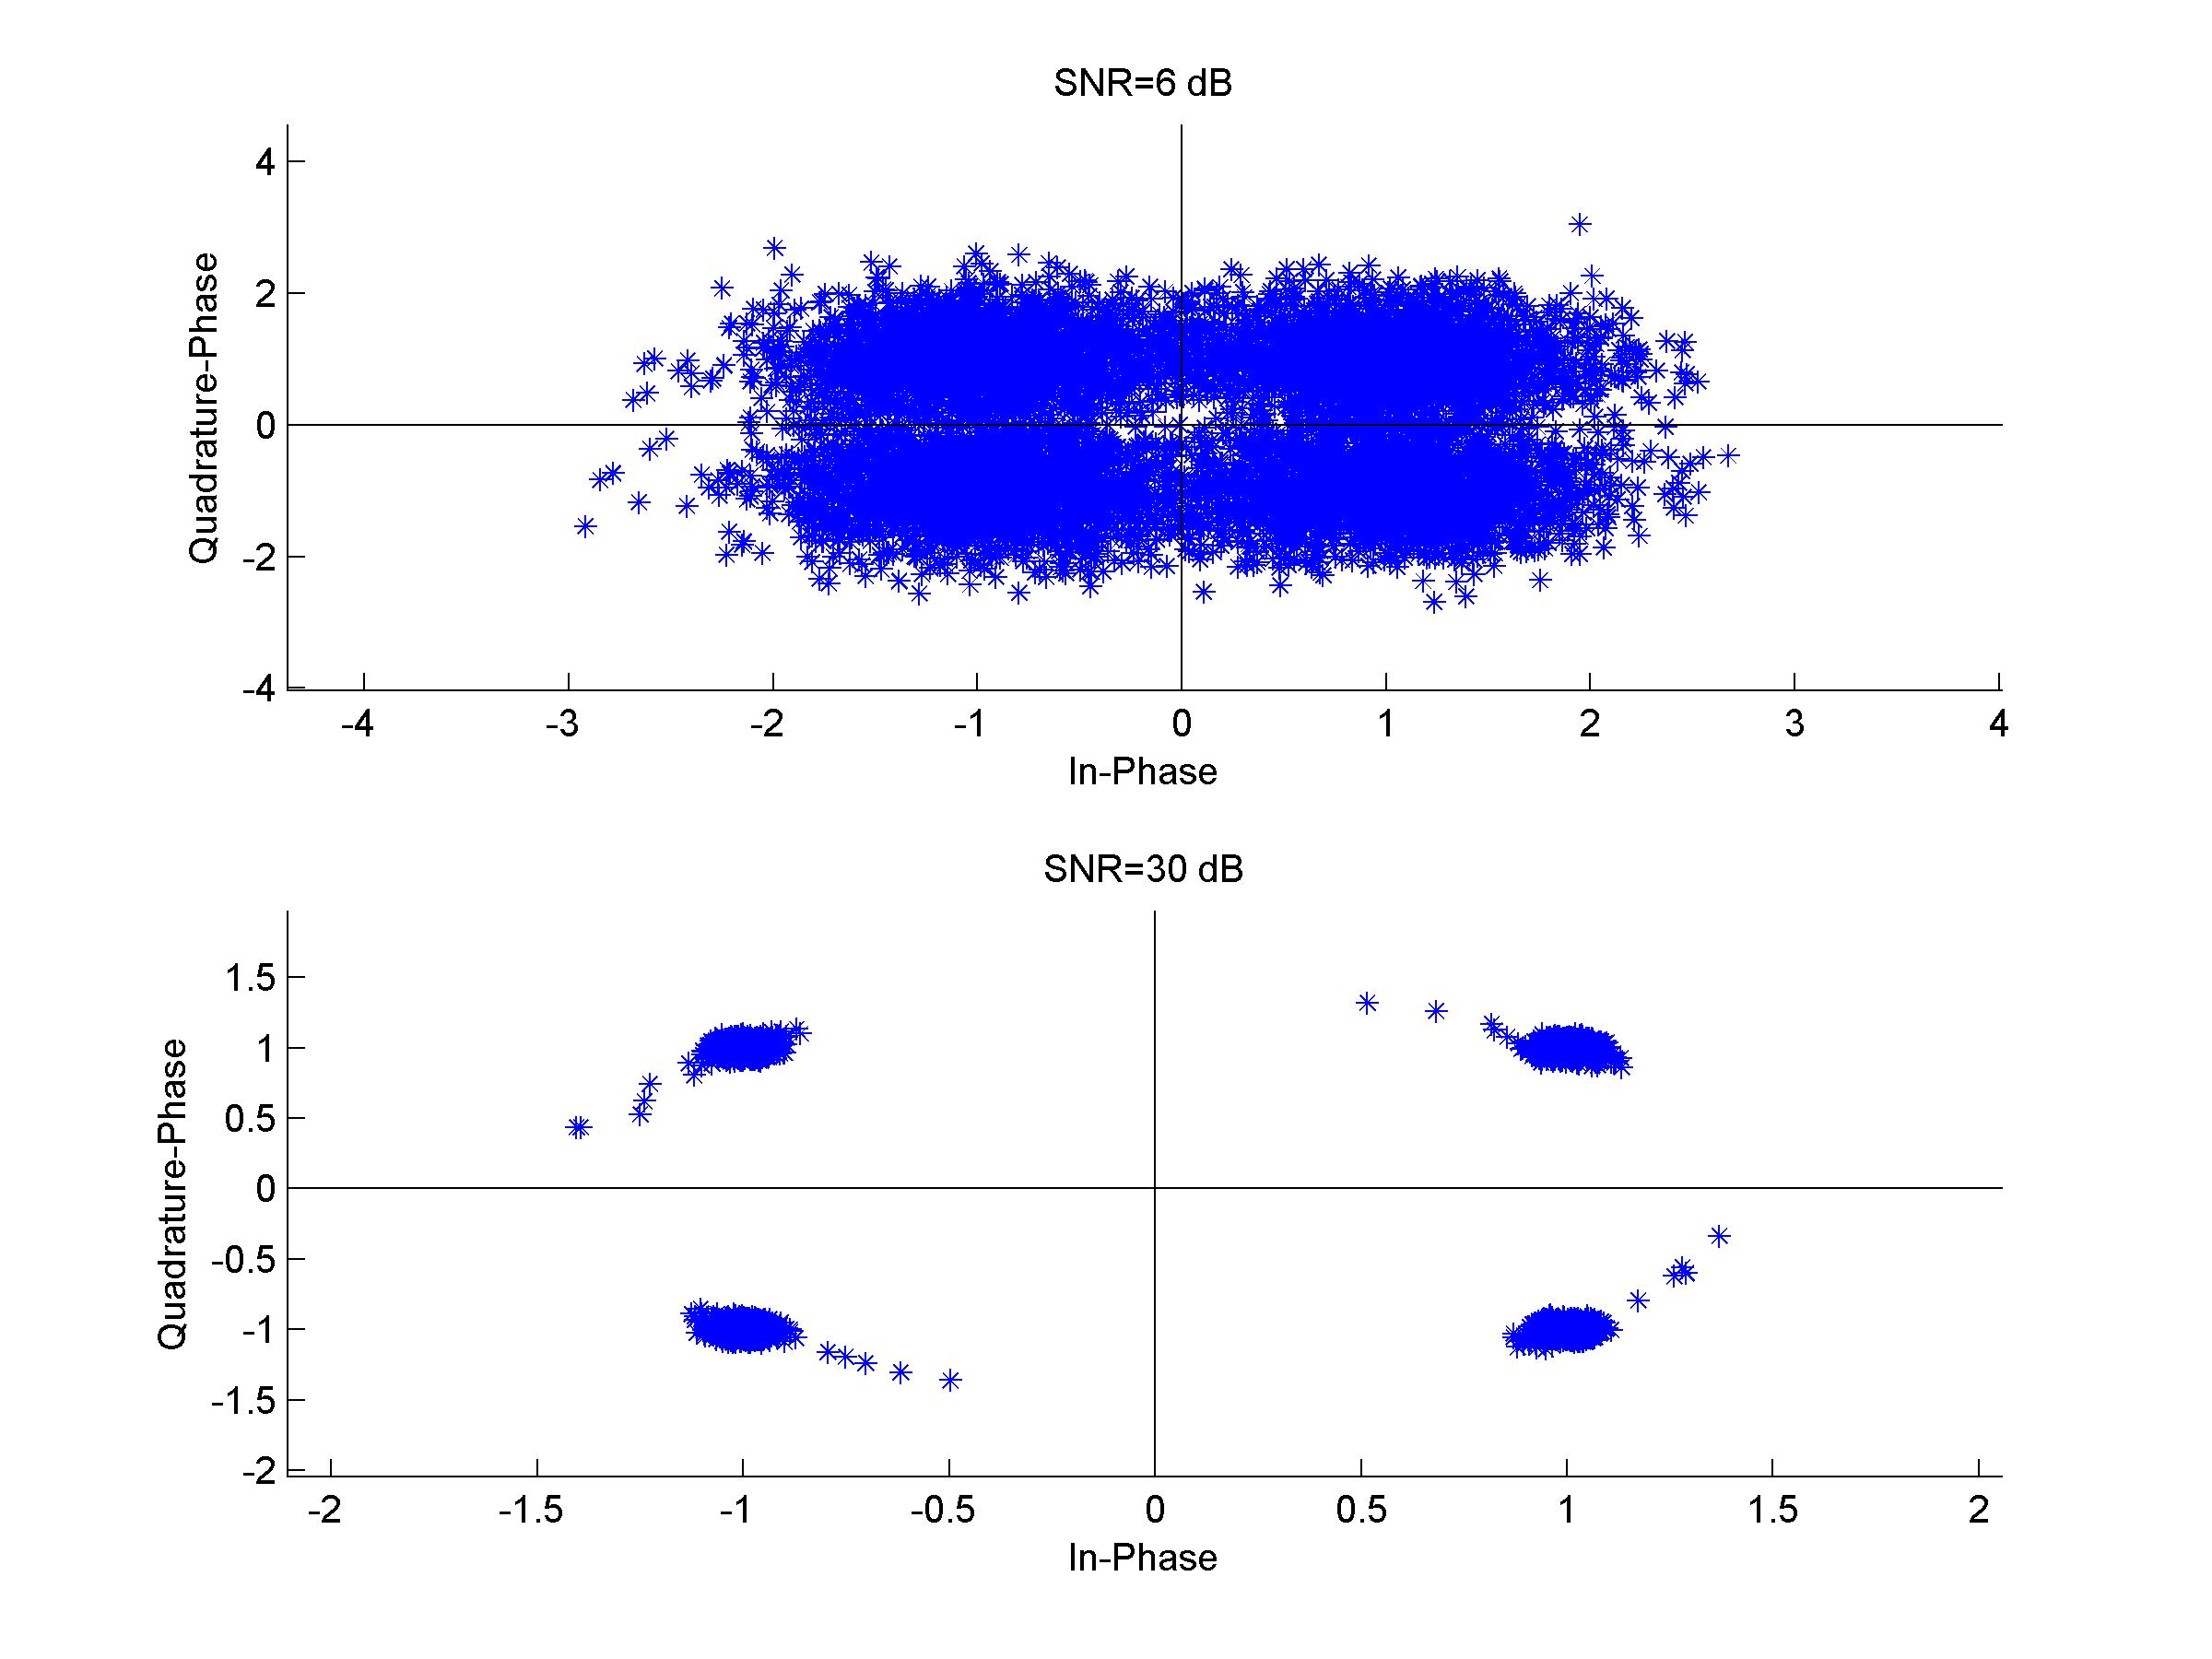
\includegraphics[width=0.7\textwidth]{qpConstpo_ddr1.jpg}
%\caption{The resulting constellation plot of the output of the system with Decision Directed Recovery Loop for an input with 30 degrees phase offset at 6dB and 30dB SNR \label{fig:ddrConstPhase}}
%\end{figure}
%
%\subsubsection{BER Plots for Phase Recovery}
%\begin{figure}[H]
%\centering
%\hspace*{-2cm}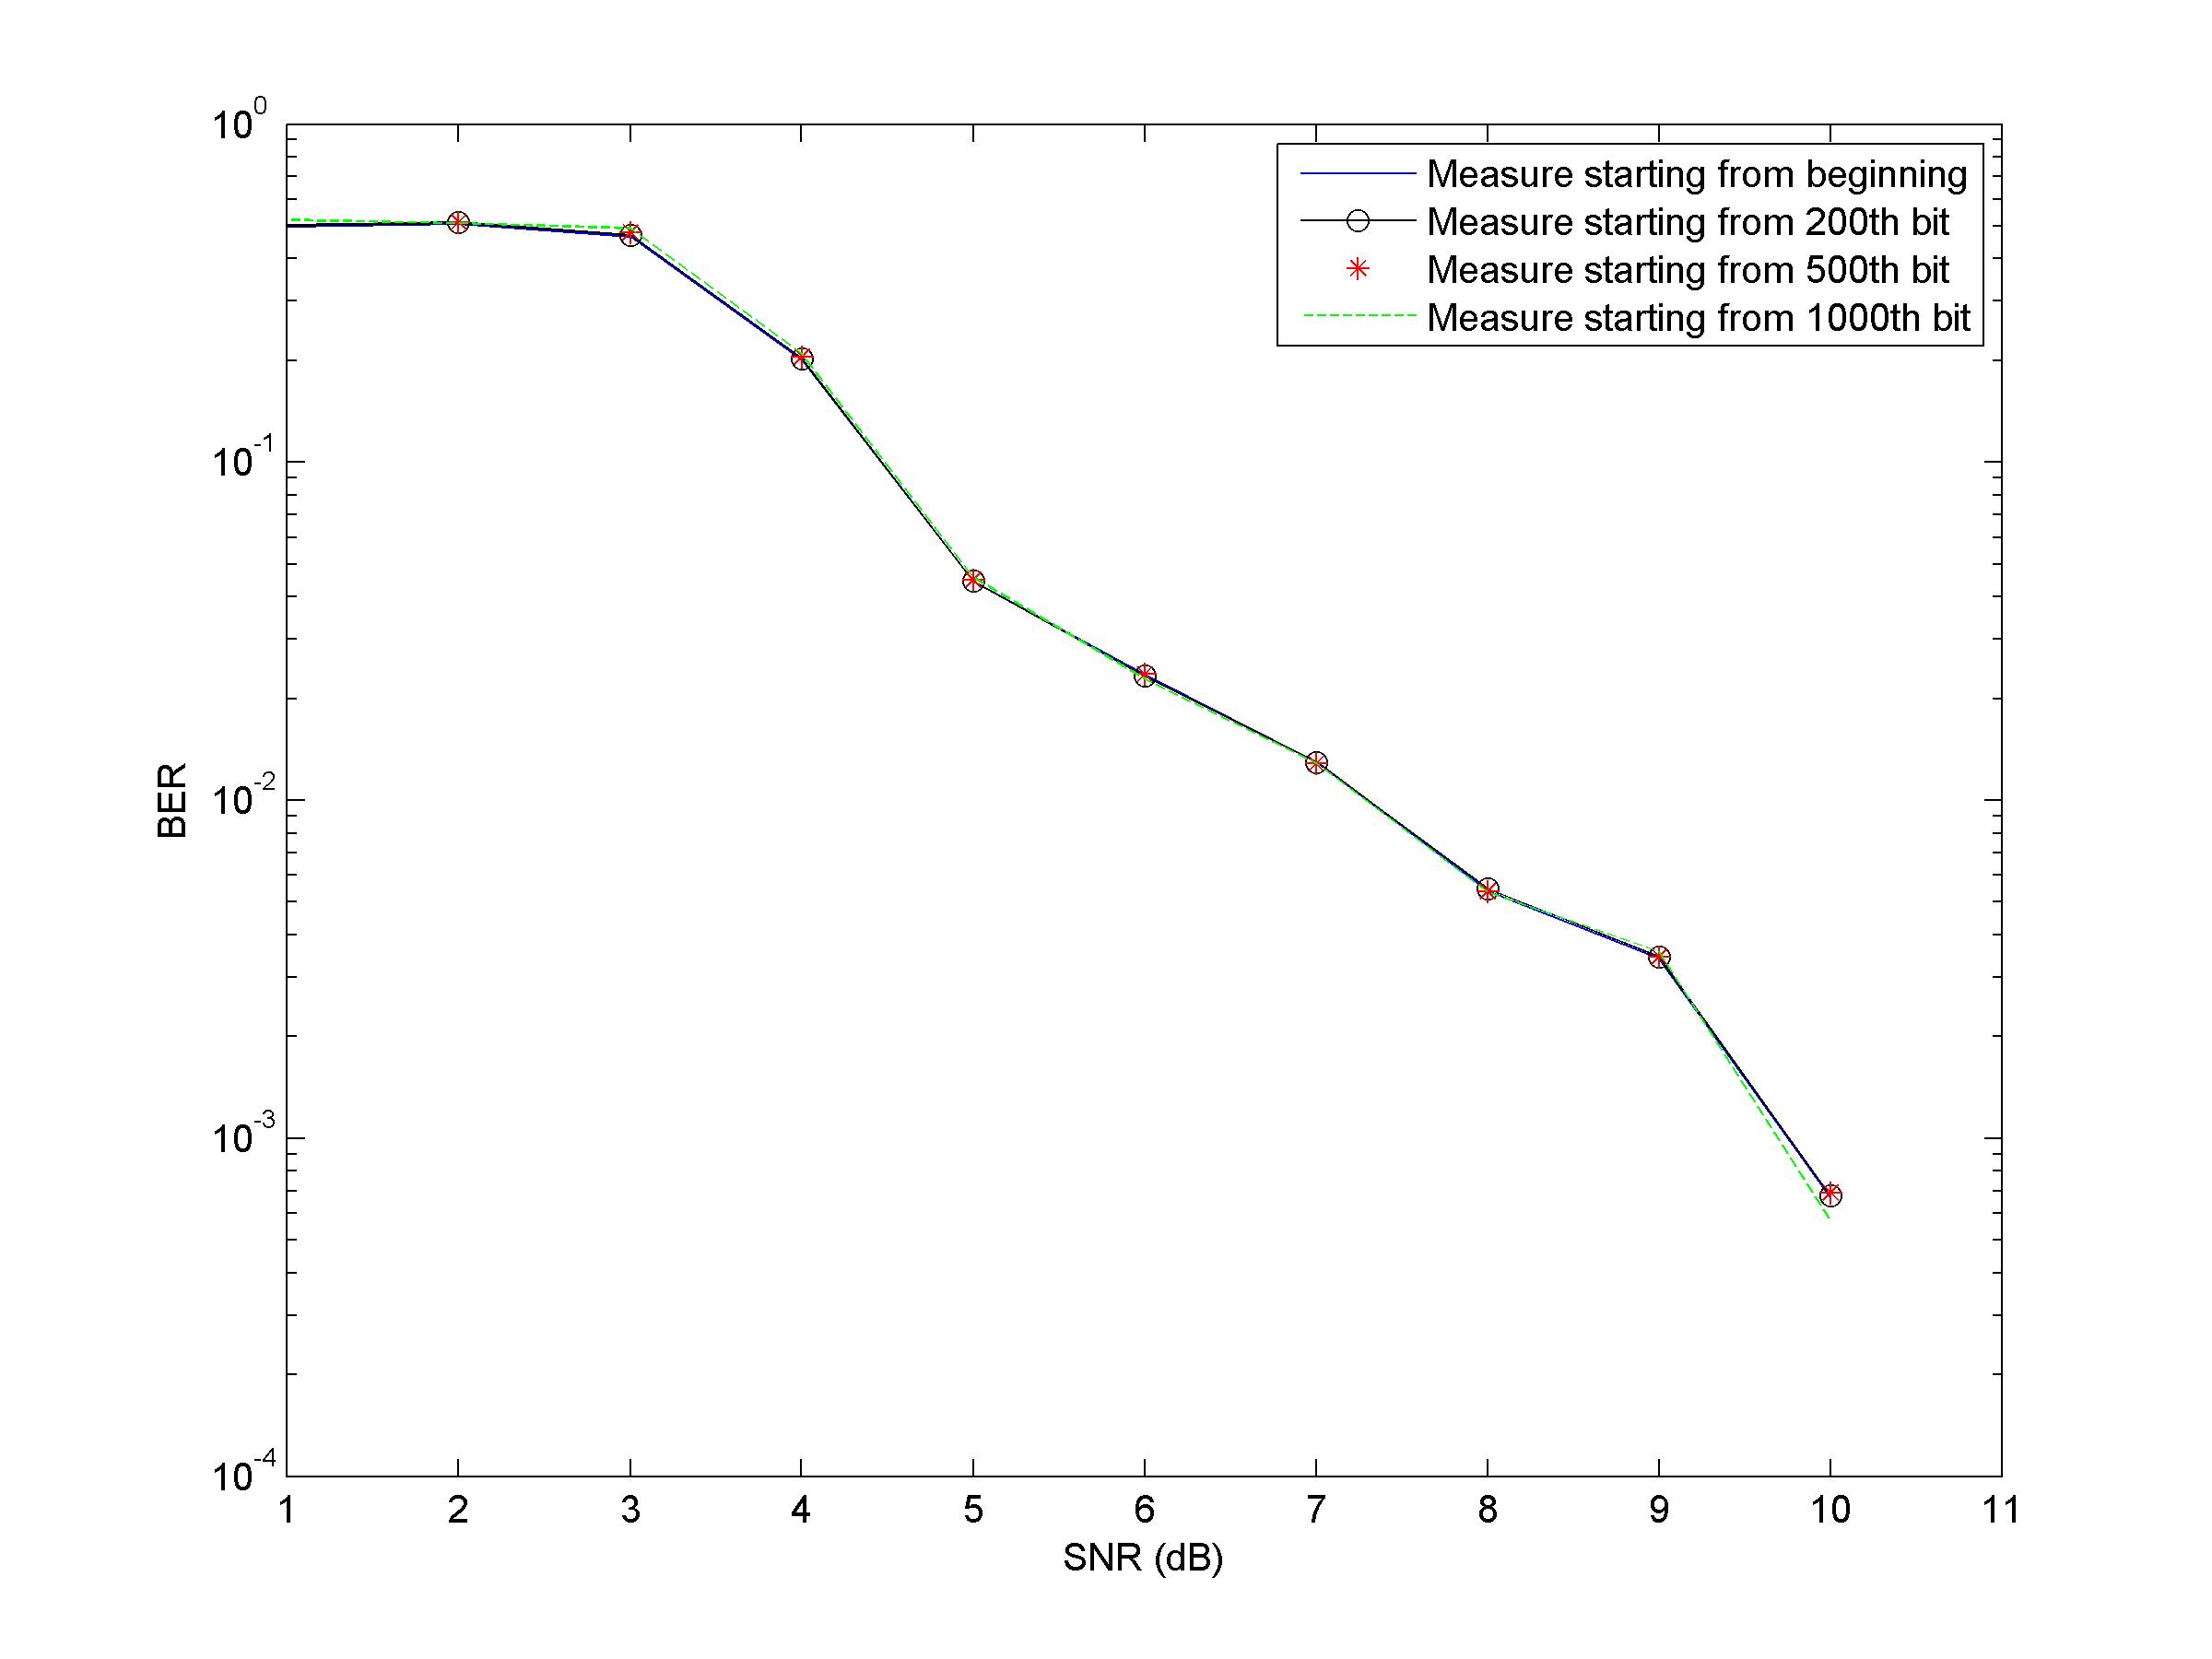
\includegraphics[width=0.7\textwidth]{qpBERpo_ddr1.jpg}
%\caption{BER plots of the system with Decision Directed Recovery Loop for an input with 30 degrees phase offset (using output bits starting from different indexes) \label{fig:ddrBERphase}}
%\end{figure}
%
%\subsubsection{BER Plots for Carrier Recovery}
%\begin{figure}[H]
%\centering
%\hspace*{-2cm}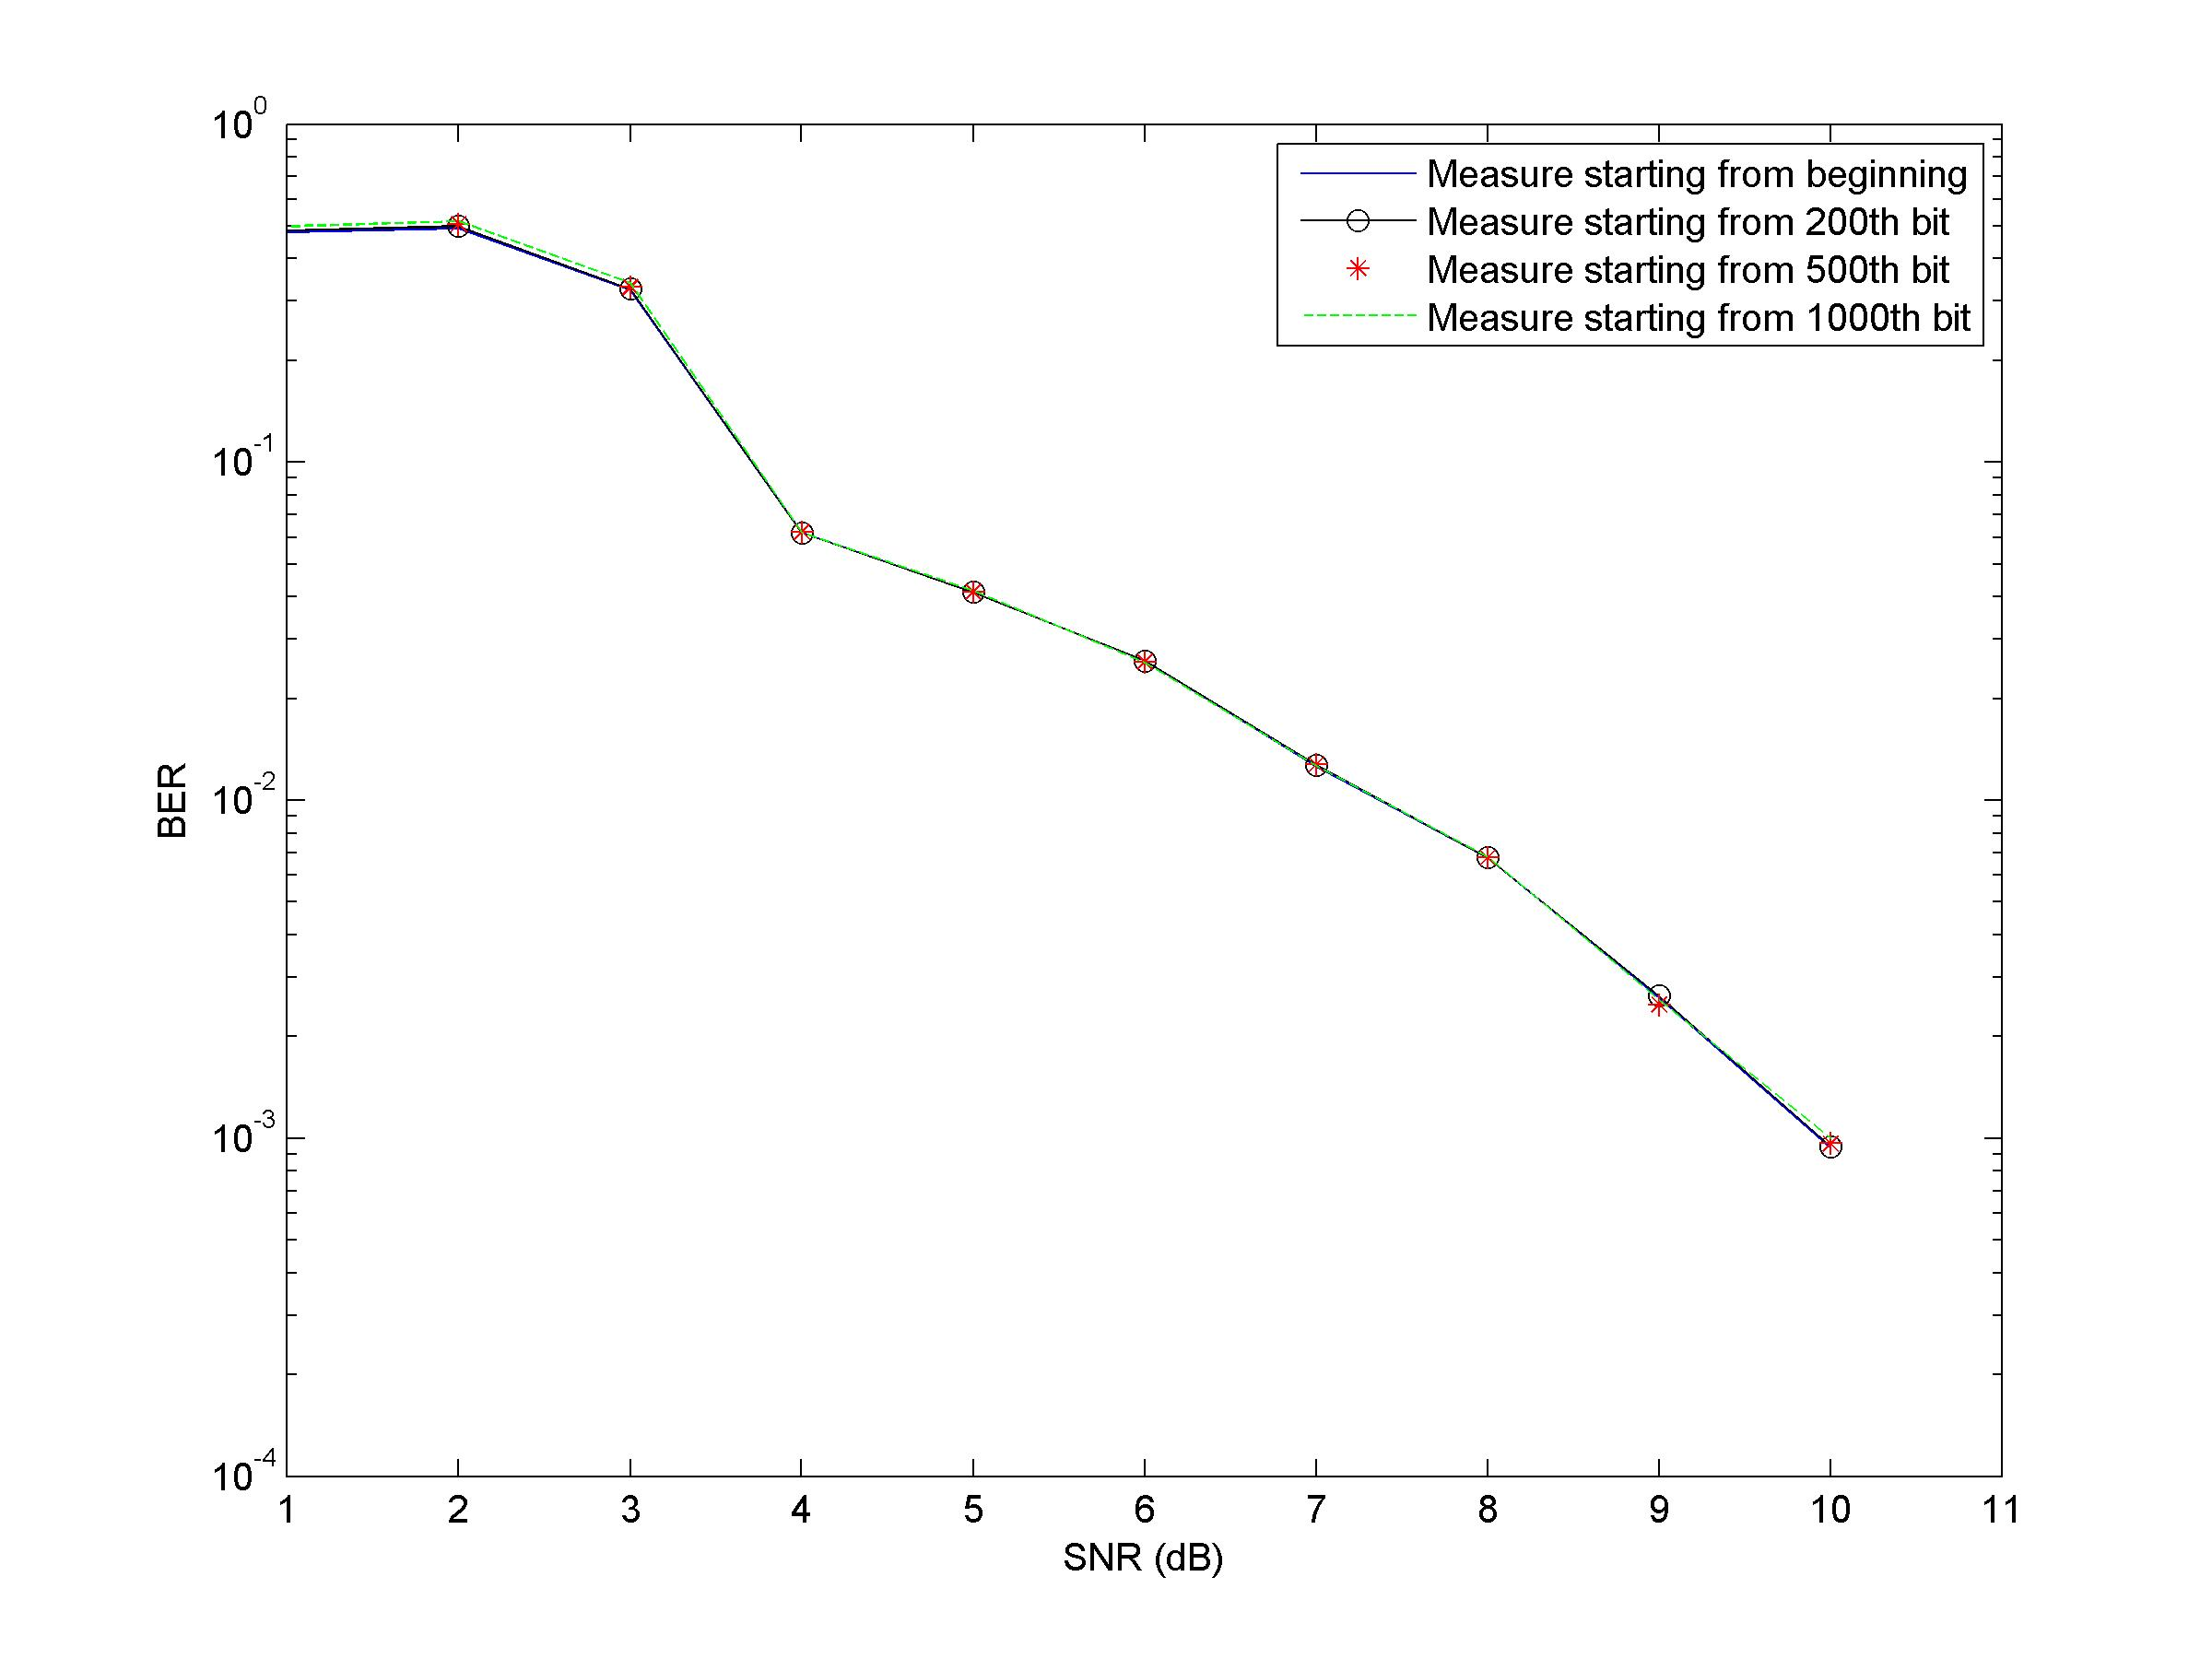
\includegraphics[width=0.7\textwidth]{qpBERfo_ddr1.jpg}
%\caption{BER plots of the system with Decision Directed Recovery Loop for an input with 1ppm frequency offset (using output bits starting from different indexes) \label{fig:ddrBERFreq1}}
%\end{figure}


\newpage
\section{Conclusion}
\label{sec:conc}

The objective of this step was to recover the system from the phase and frequency offsets that might be present in the received signal. To handle the noncoherent error introduced into the system, feedback loops (Costas and Decision Directed) were installed. These use control feedback to track out the errors by first finding a metric for the error, then using integrators to track away that error. 

The `S' Curve results for the Costas type setup give indication of how the system reacts to different degree phase and frequency error.  Notice, in each of the graphs [\ref{fig:costasSphase}, \ref{fig:costasSfreq}], the estimation error is periodic.  This is because the the metric does a good job approximating for phase at small phase levels, but of course has some error.  We see the same results in the Decision Directed cases as well [\ref{fig:ddrsphase}, \ref{fig:ddrsfreq}].

In the transience plots, notice that the error in the 6 dB is zero mean and has magnitude around .01.  The 30 dB plot [\ref{fig:costasTransPhase}]  shows the typical convergence shape we would expect.  We feel that the same structure exists in the lower SNR case, but the settling time happens in only a few samples and gets lost.  This pattern is repeated for the frequency estimation trials as well [\ref{fig:costasTransFreq1}, \ref{fig:costasTransFreq2}].  Again, the Decision Directed loops have the same form [\ref{fig:ddrTransphase}, \ref{fig:ddrtransFreq1}, \ref{fig:ddrTransFreq2}].

The constellation plots are also informative.  Note how in the Phase Costas Loop, Figure~\ref{fig:costasConstPhase}, there are a few points that have the stretching characteristic of phase error.  Then the blurring stops and the loop locks on, creating the clumps for the symbols.  This same tracking happens in the Decision Directed constellation [\ref{fig:ddrConstPhase}].  The frequency offsets never show this tracking, perhaps because they get locked on so quickly the tail never appears.

Looking at the loop filter output results for the system where a phase offset is introduced, it can be seen that phase error estimate converges to zero very fast. This means that we don't really need to throw any of the received bits. This result can also be deduced from the BER graphs provided in the results section. When a phase offset is introduced, dropping bits doesn't really change the resulting probability of error of the system. Thus we can conclude that if the phase error estimate converges fast enough dropping bits doesn't really affect the efficiency of the system in term of bit error rate. 

The same results are valid for the system with frequency offset too, as the frequency error estimate reaches the steady-state fast enough that dropping bits doesn't really change the bit error rate of the system. 

\appendix
\newpage
\bibliographystyle{plain}
\bibliography{step4}
\newpage
%% the \\ insures the section title is centered below the phrase: Appendix B
%\section{Project Assignment}
%\label{app:assign}
%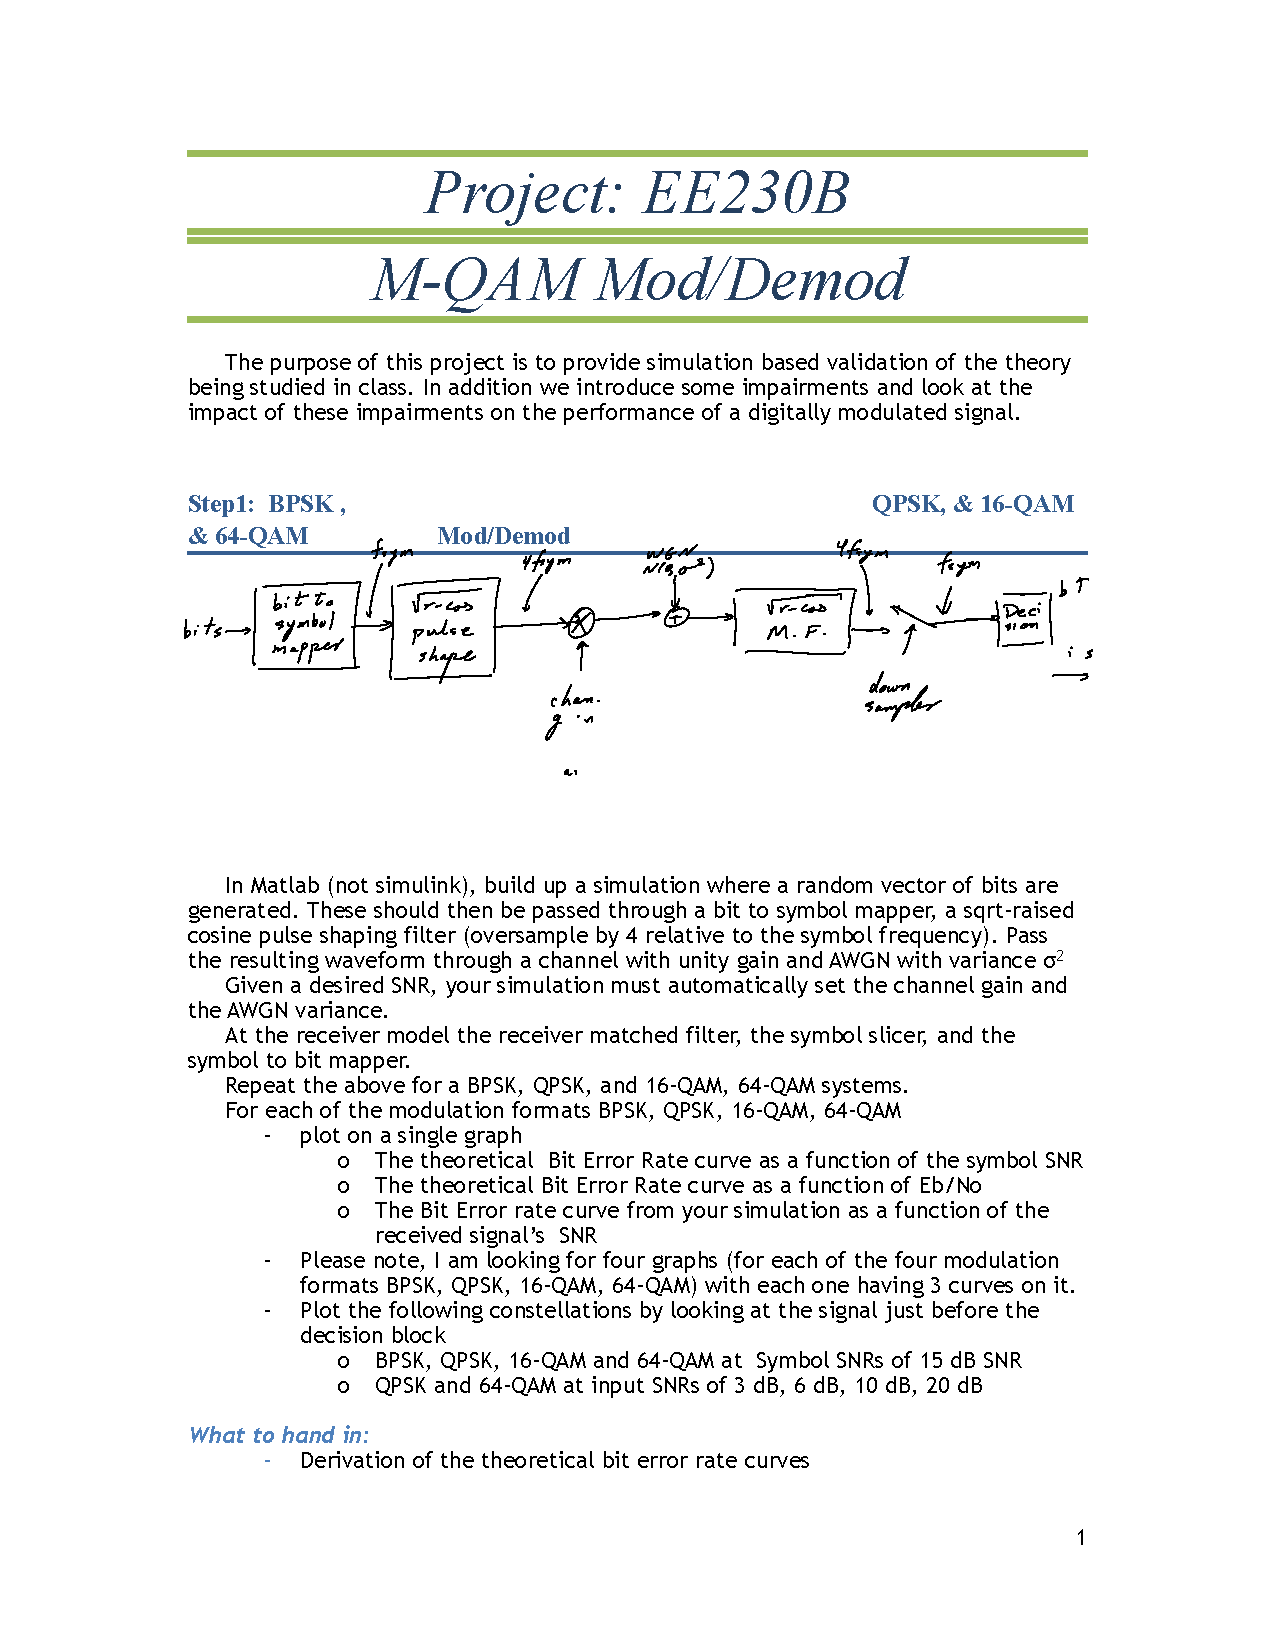
\includepdf[pages={1-5}]{project_overview.pdf}
%\cleardoublepage
%\newpage

\section{Random Bit Sequence Generator}
\label{app:random_bit_generator}
\lstinputlisting{random_bit_generator.m}

\section{Bit to Symbol Mapper}
\label{app:bittosym}
\subsection{QPSK Modulation}
\label{app:qpsk_mod}
\lstinputlisting{qpsk_mod.m}

\section{Up Sampler}
\label{app:impulse_train}
\lstinputlisting{impulse_train.m}

\section{Square Root Raised Cosine Filter}
\label{app:sqrt_raised_cosine}
\lstinputlisting{sqrt_raised_cosine.m}

\section{Additive Gaussian White Noise Channel}
\label{app:awgn_channel}
\lstinputlisting{awgn_complex_channel.m}

\section{Sampler}
\label{app:sampler}
\lstinputlisting{sampler.m}

\section{Decision Block}
\label{app:dblocks}
\subsection{QPSK Demodulation}
\label{app:qpsk_demod}
\lstinputlisting{qpsk_demod.m}

\section{Butterworth Filter}
\label{app:butterworth}
\lstinputlisting{ButterworthFilter.m}

\section{Conversion}
\label{app:convert}
\subsection{Analog-to-Digital Converter}
\label{app:ad}
\lstinputlisting{AD_conv.m}
\subsection{Digital-to-Analog Converter}
\label{app:da}
\lstinputlisting{DA_conv.m}

\subsection{Zero Hold}
\label{app:zero}
\lstinputlisting{ZeroHoldDecimation.m}
\lstinputlisting{ZeroHoldInterpolation.m}

\end{document}